\documentclass{article}
\usepackage[margin=2.5cm]{geometry}
\usepackage{graphicx}

\title{Short Report for the Course Bildverarbeitung 103-0274-01L FS22}
\author{Daniel Pfister}
\date{\today}
\graphicspath{{../images/}  {../results/}}

\begin{document}
    \maketitle
    \section{Fouriertransformation}
    \subsection{Transformation}
    \begin{figure}[h]
        \centering
        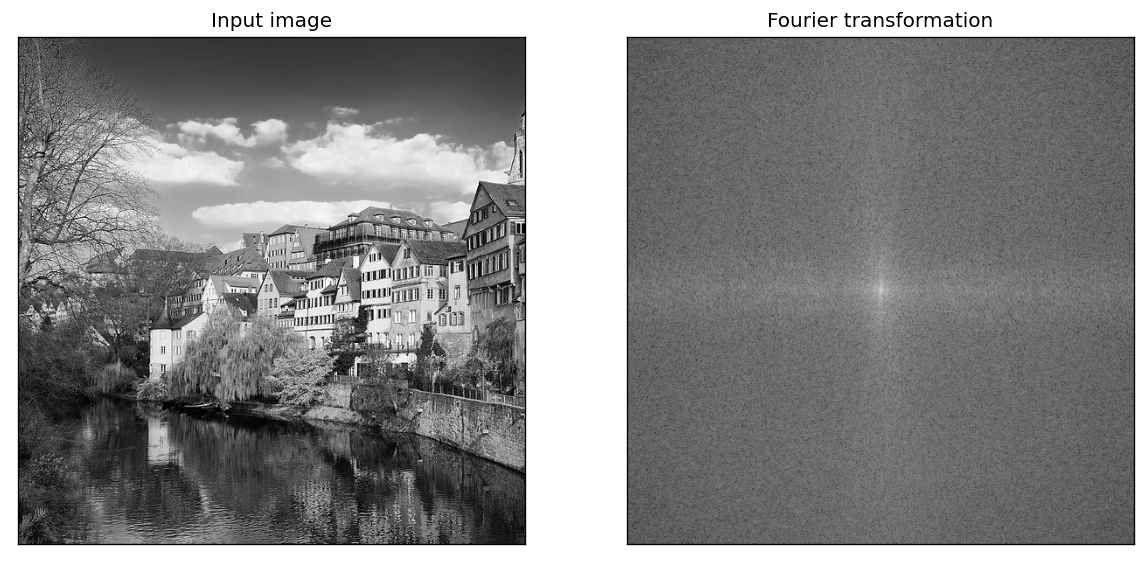
\includegraphics[width = 0.75\textwidth]{fft_1}
        \caption{the input image and its Fouriertransform}
        \label{fig:fft_1}
    \end{figure}
    Figure \ref{fig:fft_1} shows the input image on the left and the spectrum after applying \verb|scipy.fft.fft2| and shifting it using \verb|scipy.fft.fftshift|.
    \subsection{High-pass filter}
    \begin{figure}[h]
        \centering
        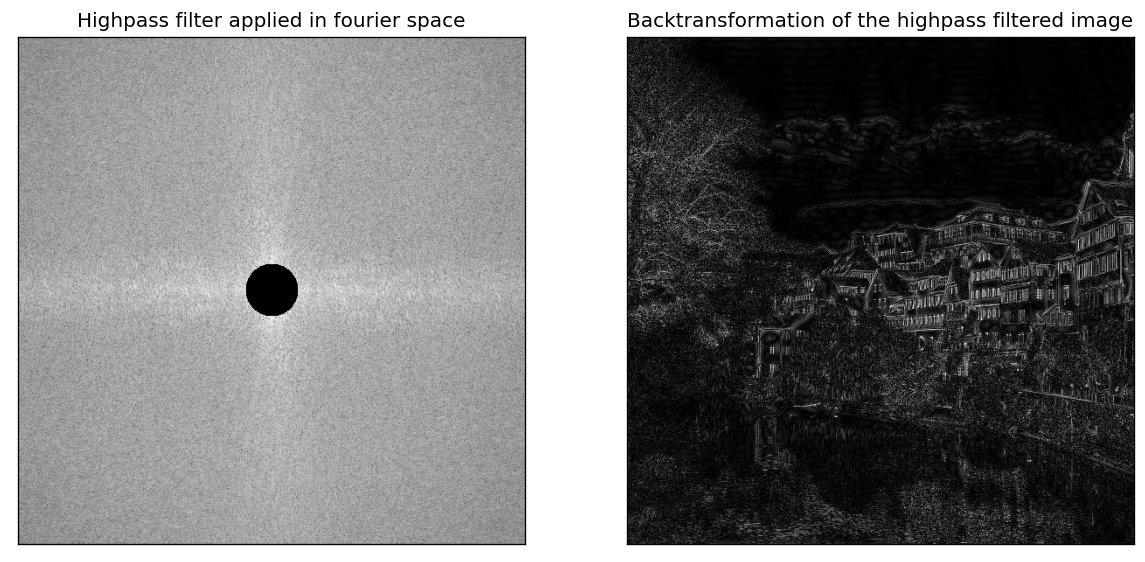
\includegraphics[width = 0.75\textwidth]{highpassfilter.png}
    \end{figure}
\end{document}